\documentclass[aspectratio=169]{beamer}

%
% Choose how your presentation looks.
%
% For more themes, color themes and font themes, see:
% http://deic.uab.es/~iblanes/beamer_gallery/index_by_theme.html
%
\mode<presentation>
{
  \usetheme{default}      % or try Darmstadt, Madrid, Warsaw, ...
  \usecolortheme{default} % or try albatross, beaver, crane, ...
  \usefonttheme{default}  % or try serif, structurebold, ...
  \setbeamertemplate{navigation symbols}{}
  \setbeamertemplate{caption}[numbered]
  \setbeamertemplate{footline}[page number]
  \setbeamercolor{frametitle}{fg=white}
  \setbeamercolor{footline}{fg=black}
} 

\usepackage[english]{babel}
\usepackage[utf8x]{inputenc}
\usepackage{tikz}
\usepackage{listings}
\usepackage{courier}
\usepackage{bold-extra}
\usepackage{minted}

\usemintedstyle{\small}

\xdefinecolor{darkblue}{rgb}{0.1,0.1,0.7}
\xdefinecolor{dianablue}{rgb}{0.18,0.24,0.31}
\definecolor{commentgreen}{rgb}{0,0.6,0}
\definecolor{stringmauve}{rgb}{0.58,0,0.82}

\lstset{ %
  backgroundcolor=\color{white},      % choose the background color
  basicstyle=\ttfamily\small,         % size of fonts used for the code
  breaklines=true,                    % automatic line breaking only at whitespace
  captionpos=b,                       % sets the caption-position to bottom
  commentstyle=\color{commentgreen},  % comment style
  escapeinside={\%*}{*)},             % if you want to add LaTeX within your code
  keywordstyle=\color{blue},          % keyword style
  stringstyle=\color{stringmauve},    % string literal style
  showstringspaces=false,
  showlines=true
}

\lstdefinelanguage{scala}{
  morekeywords={abstract,case,catch,class,def,%
    do,else,extends,false,final,finally,%
    for,if,implicit,import,match,mixin,%
    new,null,object,override,package,%
    private,protected,requires,return,sealed,%
    super,this,throw,trait,true,try,%
    type,val,var,while,with,yield},
  otherkeywords={=>,<-,<\%,<:,>:,\#,@},
  sensitive=true,
  morecomment=[l]{//},
  morecomment=[n]{/*}{*/},
  morestring=[b]",
  morestring=[b]',
  morestring=[b]"""
}

\title[2016-09-15-strangeloop]{\sc \large \textcolor{black}{making histograms functional}}
\author{\textcolor{darkblue}{Jim Pivarski}}
\institute{\textcolor{darkblue}{Princeton University -- DIANA-HEP}}
\date{\textcolor{darkblue}{September 15, 2016}}

\begin{document}

\logo{\pgfputat{\pgfxy(0.11, 7.4)}{\pgfbox[right,base]{\tikz{\filldraw[fill=dianablue, draw=none] (0 cm, 0 cm) rectangle (50 cm, 1 cm);}
\includegraphics[height=1 cm]{diana-hep-logo.png}}}}

\begin{frame}
  \vspace{1.25 cm}
  \begin{center}
    
\includegraphics[width=0.6\linewidth]{histogrammar-logo.png}
  \end{center}

  \vspace{-1.25 cm}
  \titlepage
\end{frame}

% Uncomment these lines for an automatically generated outline.
%\begin{frame}{Outline}
%  \tableofcontents
%\end{frame}

\begin{frame}{Tale of two cities}
\vspace{0.2 cm}
\begin{columns}
\column{0.5\linewidth}
\begin{center}
\textcolor{darkblue}{\Large \underline{Statistical Computing}}

\vspace{0.25 cm}
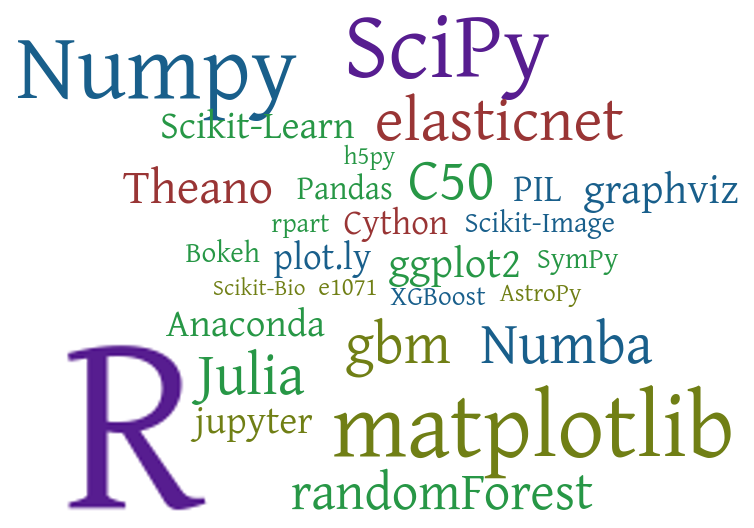
\includegraphics[height=3.5 cm]{statistical-software.png}
\end{center}

\vspace{-0.35 cm}
\begin{uncoverenv}<2->
\begin{itemize}
\item Often natively compiled, driven by high-level languages.
\item Primary customer is the laptop data analysis.
\end{itemize}
\end{uncoverenv}

\column{0.5\linewidth}
\begin{center}
\textcolor{darkblue}{\Large \underline{Big Data}}

\vspace{0.25 cm}
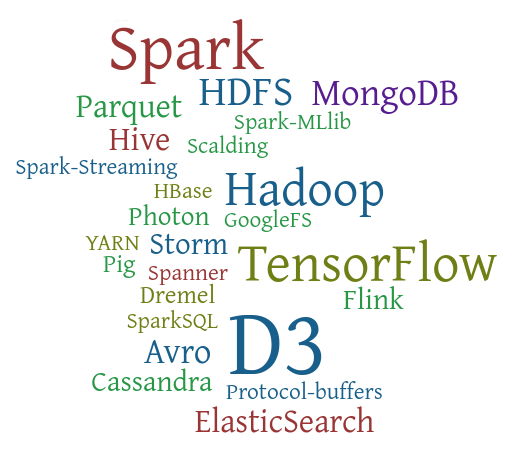
\includegraphics[height=3.5 cm]{bigdata-software.png}
\end{center}

\vspace{-0.35 cm}
\begin{uncoverenv}<3->
\begin{itemize}
\item Usually Java/Spark/Clojure.
\item More emphasis on scale-out than single-processor speed.
\item Datasets assumed to be {\it big.}
\end{itemize}
\end{uncoverenv}

\end{columns}
\end{frame}

\begin{frame}{A third you may not have heard about}
\vspace{0.5 cm}
\begin{center}
\textcolor{darkblue}{\Large \underline{High Energy Physics (HEP)}}

\vspace{0.25 cm}
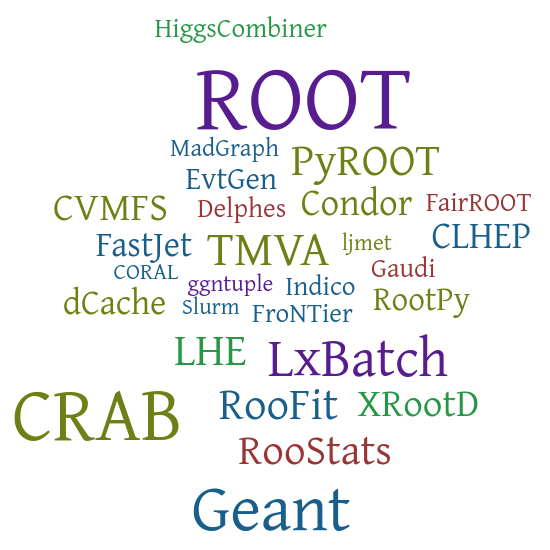
\includegraphics[height=6 cm]{hep-software.png}
\end{center}
\end{frame}

\begin{frame}{A third you may not have heard about}
\vspace{0.25 cm}
\begin{columns}
\column{0.5\linewidth}
\begin{center}
\textcolor{darkblue}{\Large \underline{High Energy Physics (HEP)}}

\vspace{0.25 cm}
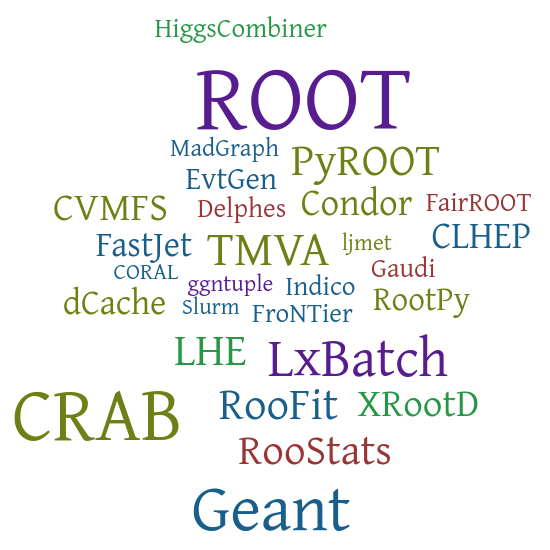
\includegraphics[height=6 cm]{hep-software.png}
\end{center}

\column{0.5\linewidth}
\begin{itemize}
\item Natively compiled, optimized for single-processor throughput.
\item<2-> {\it Throughput,} not speed: this is not High Performance Computing (HPC).
\item<3-> Datasets have always been ``big'' 
\begin{itemize}
\item<3-> SPS in 1980's: $\sim$100~GB per year
% https://www.researchgate.net/publication/275209564_UA1_Data-acquisition_System 1.6 MB/event? (``raw'')
% https://cern.ch/delfino/Generic%20LHC%20Computing%202000.ppt 0.1 MB/event (probably after processing)
% http://cerncourier.com/cws/article/cern/28849
\item<4-> LHC today: $\sim$25~PB per year
% http://www.lhc-closer.es/taking_a_closer_look_at_lhc/0.lhc_data_analysis
% https://home.cern/about/updates/2013/02/cern-data-centre-passes-100-petabytes
\end{itemize}
\end{itemize}

\vspace{0.2 cm}
\hfill \only<5>{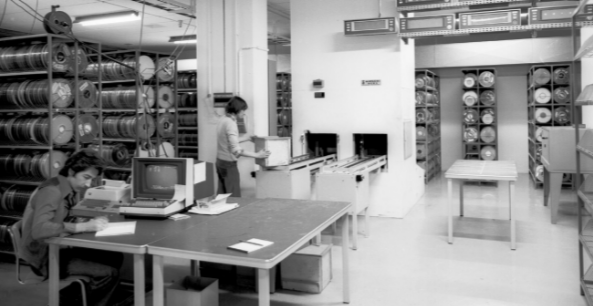
\includegraphics[width=0.87\linewidth]{tapes1.png}}\only<6>{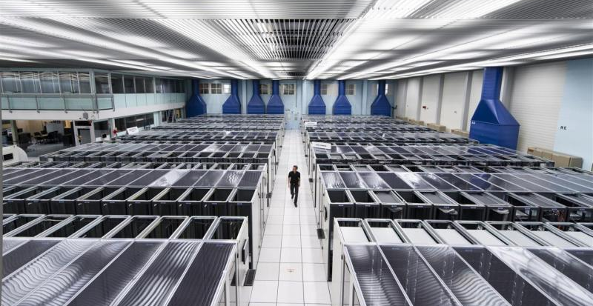
\includegraphics[width=0.87\linewidth]{cerncomputing.png}}
\vspace{-0.2 cm}
\end{columns}
\end{frame}

\begin{frame}{}
\begin{center}
\Large This community has traditionally been isolated; \\
the problems viewed as unique.

\vspace{0.5 cm}
\uncover<2->{That is no longer true.}
\end{center}

\begin{columns}
\column{0.4\linewidth}
\begin{uncoverenv}<3->
\begin{itemize}
\item HEP software needs clearly overlap with the Scipy/R/ Scikit-Learn world and the Spark/Hadoop/NoSQL world. \\ \mbox{ }
\end{itemize}
\end{uncoverenv}

\column{0.4\linewidth}
\begin{uncoverenv}<4->
\begin{itemize}
\item Individual physicists and projects like DIANA-HEP \\ (my job) are starting to explore and develop these connections.
\end{itemize}
\end{uncoverenv}

\end{columns}
\vspace{-1.5 cm}
\end{frame}

\begin{frame}{}
\vspace{1 cm}
\begin{center}
\large Considering how much has been developed on both sides of the divide, \\ small ``glue projects'' connecting them can yield a huge benefit.
\end{center}

\vspace{1 cm}
\mbox{\hspace{-1.2 cm}}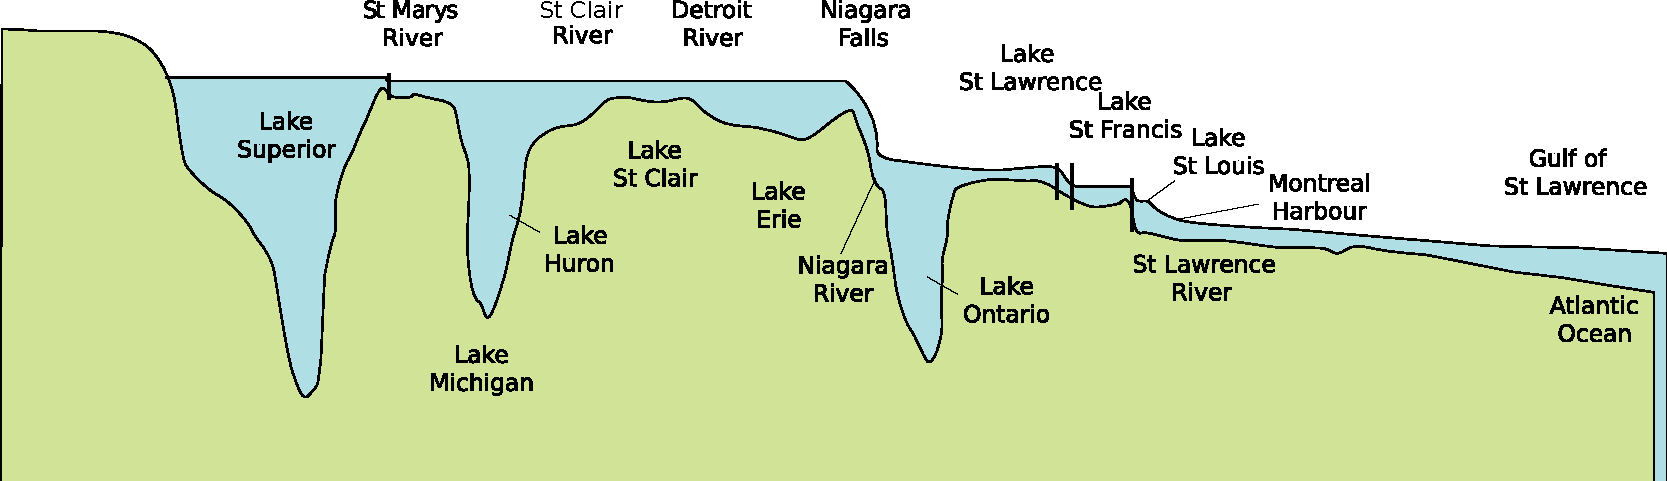
\includegraphics[width=1.16\linewidth]{great_lakes_levels.pdf}
\vspace{-1 cm}
\end{frame}

\begin{frame}{Taxonomy of the Revolution}
\vspace{0.25 cm}
\begin{columns}[t]
\column{0.33\linewidth}
\textcolor{darkblue}{\underline{Type I:}} HEP software that serves {\it the same function} as software in the wider community.

\begin{uncoverenv}<2->
\begin{center}

\includegraphics[height=1.5 cm]{stamp_replace.png}
\end{center}

Wider community has better resources for
\begin{itemize}
\item maintaining code
\item catching bugs
\item revising bad designs.
\end{itemize}
\end{uncoverenv}

\column{0.33\linewidth}
\textcolor{darkblue}{\underline{Type II:}} Domain-specific software for HEP applications. For example, ``HiggsCombiner.''

\begin{uncoverenv}<3->
\begin{center}

\includegraphics[height=1.5 cm]{stamp_keep.png}
\end{center}

Obviously. This really is a unique problem.
\end{uncoverenv}

\column{0.33\linewidth}
\textcolor{darkblue}{\underline{Type III:}} HEP software and concepts that would benefit the wider community. \\ \mbox{ }

\begin{uncoverenv}<4->
\begin{center}

\includegraphics[height=1.5 cm]{stamp_promulgate.png}
\end{center}

Cultural exchange goes both ways.
\end{uncoverenv}
\end{columns}
\end{frame}

\begin{frame}{Topic of this talk}
\begin{center}
\Large HEP histograms are an example of \textcolor{darkblue}{Type III}:

\vspace{0.5 cm}
versatile reducers for big data.
\end{center}
\end{frame}

\begin{frame}{Statistical definition of a histogram}
\vspace{0.75 cm}
A {\bf histogram} is an approximation of a distribution, formed by partitioning a sample by one of its features and counting how many items fall in each partition.

\vspace{0.25 cm}
The partitions are called {\bf bins}, and the content of each bin may be represented as the total count or the average density in that partition. \textcolor{gray}{[Start philosophical argument here.]}

\begin{center}
\only<1>{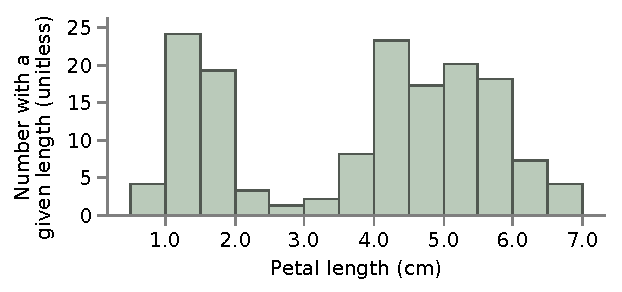
\includegraphics[width=0.7\linewidth]{Iris_Petal_Length_Histogram.pdf}}
\only<2>{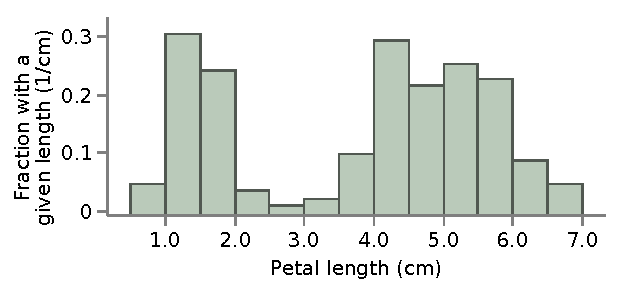
\includegraphics[width=0.7\linewidth]{Iris_Petal_Length_Histogram-2.pdf}}
\end{center}
\end{frame}

\begin{frame}[fragile]{Gallery of histogram APIs: non-HEP}
\vspace{0.25 cm}
\begin{columns}
\column{0.50\linewidth}
\begin{description}
\item[R:]

\begin{lstlisting}
hist(x, breaks =
   "Sturges", ...)
\end{lstlisting}

{\tt x} input data samples \\
{\tt breaks} binning strategy

\item[Numpy:]

\begin{lstlisting}
numpy.histogram(a, bins = 10, ...)
\end{lstlisting}

{\tt a} input data samples \\
{\tt bins} binning strategy

\item[Pandas:]

\begin{lstlisting}
DataFrame.hist(data, bins = 10, ...)
\end{lstlisting}

{\tt data} input data samples \\
{\tt bins} binning strategy
\end{description}

\column{0.51\linewidth}
\begin{description}
\item[Spark:]

\begin{lstlisting}
DoubleRDDFunctions.histogram(buckets: Array[Double])
\end{lstlisting}

{\tt this} input data samples \\
{\tt buckets} binning strategy

\item[Mathematica:]

\begin{lstlisting}
Histogram[data, hspec]
\end{lstlisting}

{\tt data} input data samples \\
{\tt hspec} binning strategy

\item[MATLAB:]

\begin{lstlisting}
histogram(X, nbins)
\end{lstlisting}

{\tt X} input data samples \\
{\tt nbins} binning strategy

\end{description}
\end{columns}

\begin{uncoverenv}<2->
\vspace{-5 cm}
\begin{center}
\fcolorbox{black}{white}{\begin{minipage}{0.8\linewidth}
\vspace{0.75 cm}
\centering They all require input data before giving you the histogram.
\vspace{0.75 cm}
\end{minipage}}
\end{center}
\vspace{5 cm}
\end{uncoverenv}
\end{frame}

\begin{frame}[fragile]{HEP histograms are different}
HEP software (HBOOK, PAW, ROOT, HippoDraw, AIDA, \ldots) treats histograms as {\it fillable containers.}

\begin{center}
\fbox{\begin{minipage}{0.6\linewidth}
\vspace{0.3 cm}
\begin{onlyenv}<1>
\vspace{0.5\baselineskip}
\hfill \begin{minipage}{0.9\linewidth}
\ttfamily\small
h = Histogram(numBins, \\
\mbox{\hspace{1.5 cm}}lowEdge, highEdge) \\
\\
for x in data: \\
\mbox{\hspace{0.75 cm}}h.fill(x) \\
\\
h.plot()
\end{minipage}
\vspace{0.5\baselineskip}
\end{onlyenv}
\begin{onlyenv}<2->
\hfill \begin{minipage}{0.9\linewidth}
\ttfamily\small
h = Histogram(numBins, \\
\mbox{\hspace{1.5 cm}}lowEdge, highEdge, "pt") \\
\\
for mu in muons: \\
\mbox{\hspace{0.75 cm}}pt = sqrt(mu.px**2 + mu.py**2) \\
\mbox{\hspace{0.75 cm}}h.fill(pt) \\
\\
h.plot()
\end{minipage}
\end{onlyenv}
\vspace{0.3 cm}
\end{minipage}}
\end{center}

\uncover<3->{This interface lets you feed in the data gradually and view partial results. \\ It presumes the dataset is too big for a single function call.}
\vspace{-0.5 cm}
\end{frame}

\begin{frame}{Everything is made out of histograms}
\vspace{0.5 cm}
\mbox{\hspace{-1.1 cm}
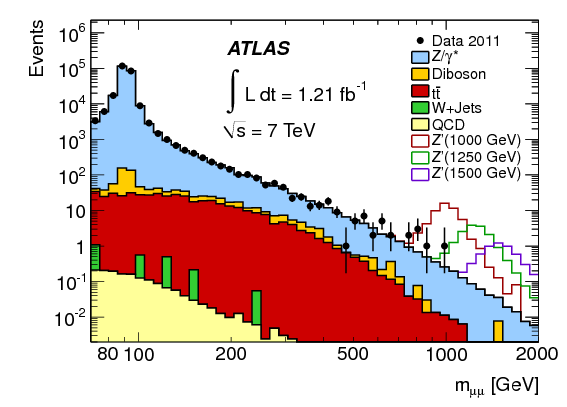
\includegraphics[height=1.8cm]{dileptons_fig_01b_mumu.png}
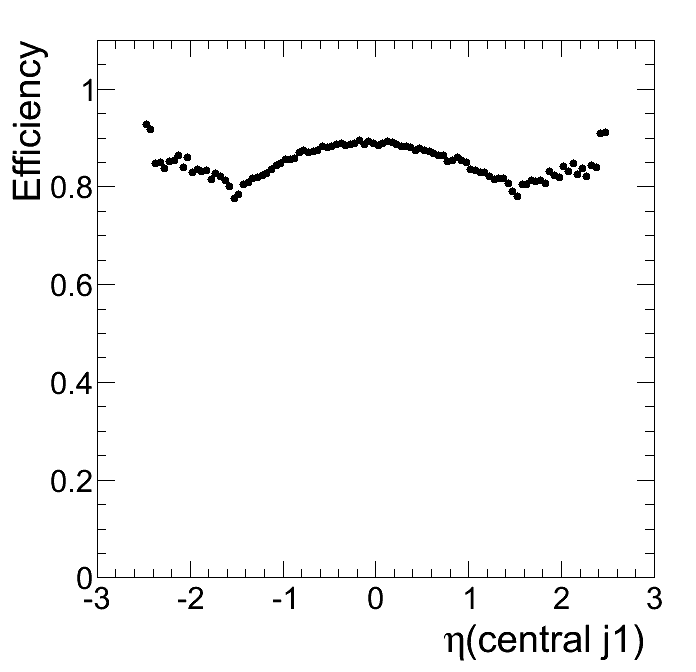
\includegraphics[height=1.8cm]{efficiency.png}
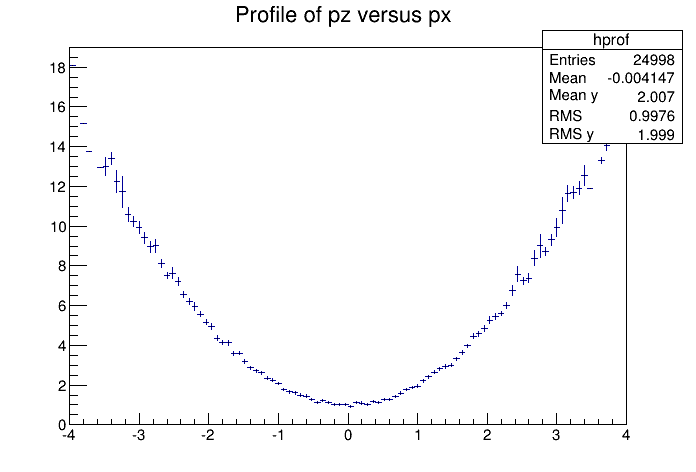
\includegraphics[height=1.8cm]{profile_plot.png}
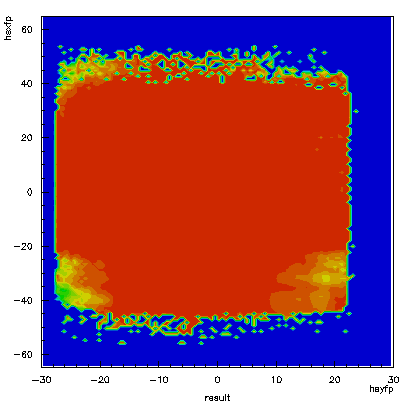
\includegraphics[height=1.8cm]{efficiency_2d.png}
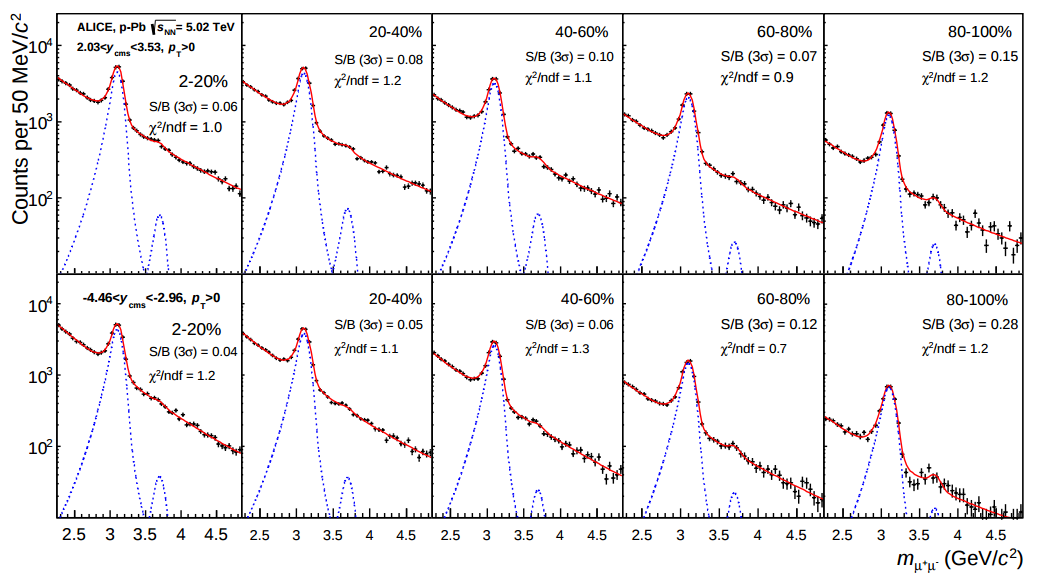
\includegraphics[height=1.8cm]{histograms_of_histograms.png}
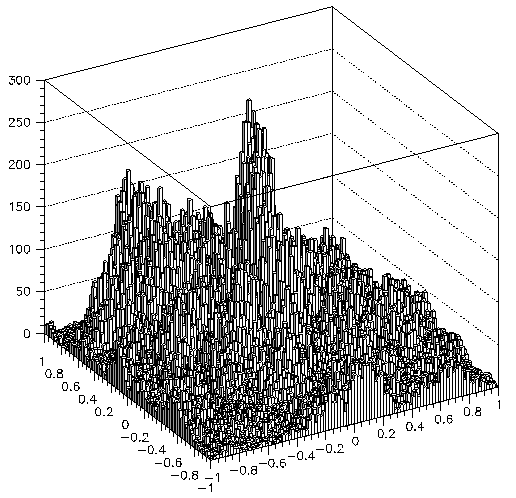
\includegraphics[height=1.8cm]{lego_plot.png}
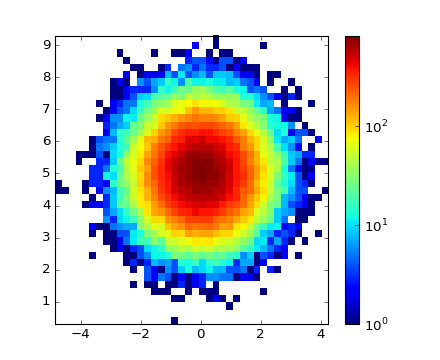
\includegraphics[height=1.8cm]{two_dimensional.png}}

\vspace{0.5 cm}
\begin{center}
\begin{minipage}{0.9\linewidth}
\Large Histograms have become the basic unit of HEP data analysis, used to make almost everything else. Analogous to

\vspace{0.5 cm}
\hspace{0.5 cm}\begin{minipage}{0.5\linewidth}
\begin{itemize}
\item lists in LISP
\item dictionaries in Python
\item data.frames in R
\end{itemize}
\end{minipage}
\end{minipage}
\end{center}
\end{frame}

\begin{frame}{Examples (only one of which is really a histogram)}
\vspace{0.5 cm}
\begin{columns}
\column{0.33\linewidth}
\mbox{ } \hfill \hfill \hfill \textcolor{darkblue}{Stacked histograms} \hfill \mbox{ }

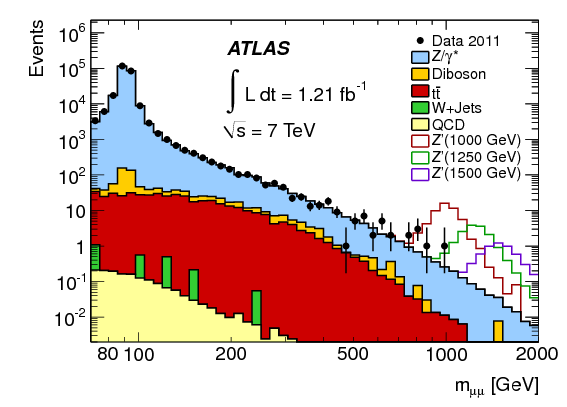
\includegraphics[height=3.5 cm]{dileptons_fig_01b_mumu.png}

Represents contributions from different samples to a total histogram.

\vspace{0.25 cm}
\begin{minipage}{\linewidth}
\scriptsize Constructed by cumulatively filling a series of histograms and overlaying them in reverse order.
\end{minipage}

\column{0.33\linewidth}
\mbox{ } \hfill \hfill \textcolor{darkblue}{Efficiency plot} \hfill \mbox{ }

\mbox{ } \hfill 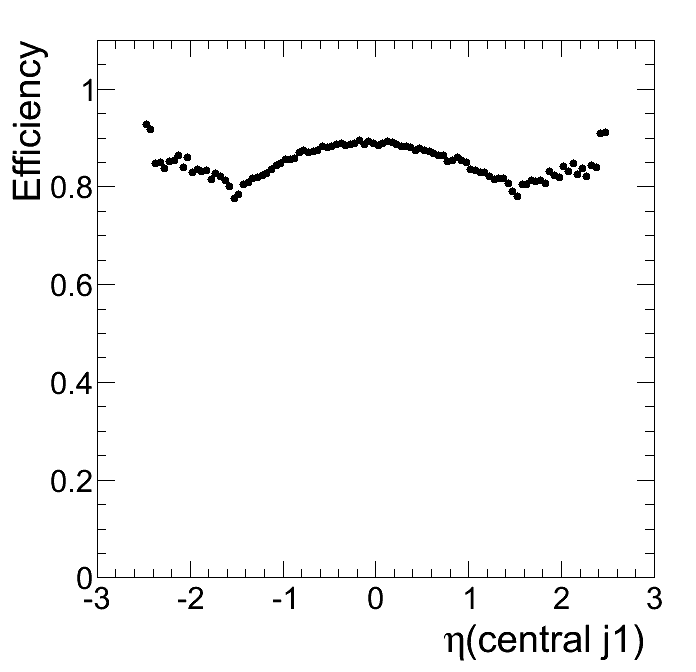
\includegraphics[height=3.5 cm]{efficiency.png} \hfill \mbox{ }

Represents the probability of passing a filter versus some variable.

\vspace{0.25 cm}
\begin{minipage}{\linewidth}
\scriptsize Constructed by filling two histograms, one with the filter, the other without, and dividing them bin-by-bin.
\end{minipage}

\column{0.33\linewidth}
\mbox{ } \hfill \textcolor{darkblue}{Profile plot} \hfill \mbox{ }

\mbox{\hspace{-0.25 cm}}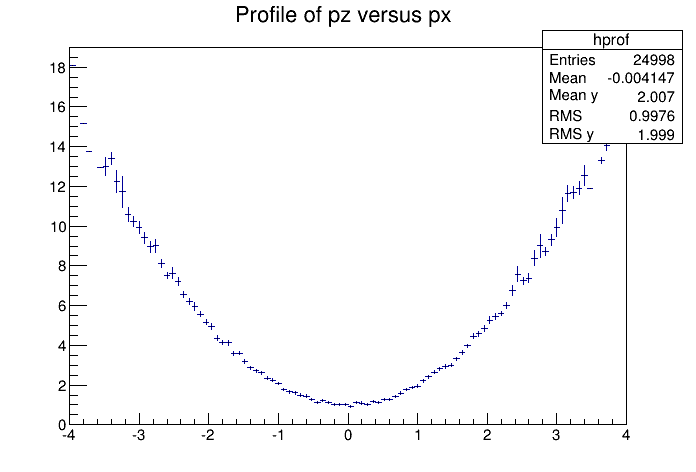
\includegraphics[height=3.5 cm]{profile_plot.png}

Represents a marginal projection of the dataset with errors on the mean.

\vspace{0.25 cm}
\begin{minipage}{\linewidth}
\scriptsize Constructed by filling $\sum_i y_i$ and $\sum_i {y_i}^2$ separately and doing the appropriate transformations bin-by-bin.
\end{minipage}
\end{columns}
\end{frame}

\begin{frame}{The problem with this API}
\vspace{0.65 cm}
\textcolor{darkblue}{Domain-specific knowledge enters in two different places: histogram-construction and histogram-filling.}

\begin{center}
\begin{minipage}{0.8\linewidth}
\vspace{0.25 cm}
$\left.\mbox{\rotatebox{90}{\hspace{-0.9 cm}construction}\hspace{0.15 cm}}\right\{\begin{array}{l}\mbox{\ttfamily\small job[N].h = Histogram(numBins, lowEdge, highEdge)} \\ \hspace{2.3 cm}\mbox{\textcolor{darkblue}{\# binning requires knowledge of the problem domain}}\end{array}$

\vspace{0.25 cm}
$\left.\mbox{\rotatebox{90}{\hspace{-0.65 cm}\hspace{0.35 cm}filling\hspace{0.35 cm}}}\hspace{0.1 cm}\right\{\begin{array}{l}\mbox{\ttfamily\small for event in job[N].physicsEvents:} \\ \mbox{\ttfamily\small \hspace{0.75 cm}job[N].h.fill(event.whatToPlot())} \\ \hspace{2.3 cm}\mbox{\textcolor{darkblue}{\# {\ttfamily\small whatToPlot()} requires knowledge of the problem domain}}\end{array}$

\vspace{0.25 cm}
$\left.\mbox{\rotatebox{90}{\hspace{-0.5 cm}merging}}\hspace{0.1 cm}\right\{\begin{array}{l}\mbox{\ttfamily\small h = job[0].h + job[1].h + job[2].h + ...}\end{array}$
\end{minipage}
\end{center}
\end{frame}

\begin{frame}[fragile]{Specifically, in Spark\ldots}
\vspace{0.5 cm}
\begin{columns}
\column{0.5\linewidth}

\textcolor{darkblue}{Imperative analysis script}
\begin{lstlisting}
x = Histogram(100, -5.0, 5.0)

for event in events:
    x.fill(event.calcX())

x.plot()
\end{lstlisting}

\column{0.52\linewidth}
\textcolor{darkblue}{Spark equivalent}
\begin{lstlisting}
x = events.aggregate(
    Histogram(100, -5.0, 5.0),
    lambda h, event:
        h.fill(event.calcX()),
    lambda h1, h2:
        h1 + h2)

x.plot()
\end{lstlisting}
\end{columns}
\end{frame}

\begin{frame}[fragile]{Specifically, in Spark\ldots}
\vspace{0.5 cm}
\begin{columns}
\column{0.5\linewidth}

\textcolor{darkblue}{Imperative analysis script}
\begin{lstlisting}
x = Histogram(100, -5.0, 5.0)
y = Histogram(100, -5.0, 5.0)

for event in events:
    x.fill(event.calcX())
    y.fill(event.calcY())

x.plot()
y.plot()
\end{lstlisting}

\column{0.52\linewidth}
\textcolor{darkblue}{Spark equivalent}
\begin{lstlisting}
x, y = events.aggregate(
    (Histogram(100, -5.0, 5.0),
     Histogram(100, -5.0, 5.0)),
    lambda h, event: (
        h[0].fill(event.calcX()),
        h[1].fill(event.calcY())),
    lambda h1, h2: (
        h1[0] + h2[0],
        h1[1] + h2[1]))

x.plot()
y.plot()
\end{lstlisting}
\end{columns}
\end{frame}

\begin{frame}[fragile]{Specifically, in Spark\ldots}
\vspace{0.5 cm}
\begin{columns}
\column{0.5\linewidth}

\textcolor{darkblue}{Imperative analysis script}
\begin{lstlisting}
x = Histogram(100, -5.0, 5.0)
y = Histogram(100, -5.0, 5.0)
z = Histogram(100, -5.0, 5.0)

for event in events:
    x.fill(event.calcX())
    y.fill(event.calcY())
    z.fill(event.calcZ())

x.plot()
y.plot()
z.plot()
\end{lstlisting}

\column{0.52\linewidth}
\textcolor{darkblue}{Spark equivalent}
\begin{lstlisting}
x, y, z = events.aggregate(
    (Histogram(100, -5.0, 5.0),
     Histogram(100, -5.0, 5.0),
     Histogram(100, -5.0, 5.0)),
    lambda h, event: (
        h[0].fill(event.calcX()),
        h[1].fill(event.calcY()),
        h[2].fill(event.calcZ())),
    lambda h1, h2: (
        h1[0] + h2[0],
        h1[1] + h2[1],
        h1[2] + h2[2]))

x.plot()
y.plot()
z.plot()
\end{lstlisting}
\end{columns}
\end{frame}

\begin{frame}[fragile]{Solution: go functional}
\vspace{0.5 cm}
\begin{center}
\fbox{\begin{minipage}{0.85\linewidth}
\vspace{0.25 cm}
\ttfamily\small\hspace{0.25 cm} h = Histogram(numBins, lowEdge, highEdge, \textbf{fillRule})
\vspace{0.25 cm}
\end{minipage}}
\end{center}

where {\ttfamily\small\textbf{fillRule}} is a function : {\it data} $\to$ $\mathbb{R}$ that specifies how to get the binnable feature from the input dataset.

\begin{uncoverenv}<2->
\vspace{0.5 cm}
All domain domain-specific knowledge is in the {\ttfamily\small\textbf{fillRule}}. The filling function may now be generic (and automated).

\begin{center}
\fbox{\begin{minipage}{0.85\linewidth}
\vspace{0.25 cm}
\ttfamily\small\hspace{0.25 cm} h.fill(datum) \hspace{1 cm}\# calls fillRule(datum) internally
\vspace{0.25 cm}
\end{minipage}}
\end{center}
\end{uncoverenv}

\begin{uncoverenv}<3->
\vspace{0.5 cm}
(In a {\it purely} functional environment, {\ttfamily\small hnew = hold.filled(datum)}.)
\end{uncoverenv}
\end{frame}

\begin{frame}[fragile]{What this looks like in Spark}
\begin{columns}
\column{0.46\linewidth}
%% \begin{lstlisting}
%% def increment(h, event):
%%     h.fill(event)
%%     return h

%% def combine(h1, h2):
%%     return h1 + h2

%% x = events.aggregate(
%%     Histogram(100, -5.0, 5.0,
%%        lambda ev: ev.calcX()),
%%     increment,
%%     combine)

%% x.plot()
%% \end{lstlisting}

\column{0.59\linewidth}
\begin{minted}{python}
class Package:
  def __init__(self, **hs):
      self.hs = hs
  def fill(self, datum):
      for h in self.hs.values():
          h.fill(datum)
  def __add__(self, other):
      return {self.hs[n] + other.hs[n]
                  for n in self.hs}

package = events.aggregate(Package(
        x = Histogram(100, -5.0, 5.0,
                lambda ev: ev.calcX()),
        y = Histogram(100, -5.0, 5.0,
                lambda ev: ev.calcY()))
    increment, combine)

package.hs["x"].plot()
\end{minted}
\end{columns}
\end{frame}



\end{document}
